%!TEX root = ../thesis.tex
%*******************************************************************************
%****************************** Fourth Chapter *********************************
%*******************************************************************************
\chapter{Determinants of cross-tissue cell type identity and distribution} \label{chap:CT_bio}

% **************************** Define Graphics Path **************************
\ifpdf
    \graphicspath{{Chapter4/Figs/Raster/}{Chapter4/Figs/PDF/}{Chapter4/Figs/}}
\else
    \graphicspath{{Chapter4/Figs/Vector/}{Chapter4/Figs/}}
\fi
Cell identity can be defined by the genes it expresses. A continuously increasing number of studies has applied scRNA-seq to profile cells from various body locations and describe the cells that make up a tissue, in the steady-state or disease. A smaller number of studies have focused on the differences between the cell types detected in different tissues~\citep{miragaia_single-cell_2019,scott_transcription_2018}. However, we don't yet know how variable transcriptome of most cell types is between tissues, and how it relates to the tissue transcriptome.

This Chapter outlines the construction of a human cell type reference based on single-cell transcriptomics, by applying the \textit{CellTypist} framework presented in Chapter~\ref{chap:CT_method}. It will be demonstrated how this reference can be used for automatic classification of newly generated data and discuss its current advantages and limitations. The present Chapter will also focus on the interpretability of this pipeline, and reveal the genes driving cell identity across tissues. We will further dissect the relationships across tissues established by \textit{CellTypist}, and explore the influence of different cell types in tissue biology.

The work presented in this Chapter was partly developed with the assistance of Ni Huang, who contributed to the collection and integration of published datasets. The analyses here performed are based on the methodology outlined in Chapter~\ref{chap:CT_method}.


\section{Introduction}
\label{section4.1}




\section{Results}
\label{section4.2}
\subsection{Human data collection and organisation}
\label{section4.2_coll}
To obtain a global, cross-tissue perspective of human cell types, we obtained a broad representation of single-cell transcriptomes with by collecting several publicly available scRNA-seq datasets (Table~\ref{table:tab_4_1}). Information about tissue, scRNA-seq protocol, sampling method, and cell type annotation (when available) were obtained from the respective publications and data repositories, together with the gene expression matrices.

% table: Dataset; number of cells; ref
\begin{table}[ht!] % p for putting it in the next page available
\footnotesize
\caption[Datasets collected and references]{Datasets collected and references}
\centering
\label{table:tab_4_1}

\begin{tabular}{l|c|r}
\toprule
~\textbf{Dataset} & ~\textbf{Reference} & ~\textbf{\# cells} \\
\midrule
baron16 & ~\citep{baron_single-cell_2016} & 8.569  \\

bjorklund16 & ~\citep{bjorklund_heterogeneity_2016} & 648  \\

gierahn17 & ~\citep{gierahn_seq-well:_2017} & 3.694  \\

guo18 & ~\citep{guo_adult_2018} & 12.053  \\

habib17 & ~\citep{habib_massively_2017} & 14.963  \\

hcaImmune18 & \href{data.humancellatlas.org}{HCA Data Portal} & 593.844  \\

henry18 & ~\citep{henry_cellular_2018} & 109.061  \\

jaitin19 & ~\citep{jaitin_lipid-associated_2019} & 13.199  \\

james20 & \textit{Unpublished} & 32.228  \\

lamanno16 & ~\citep{la_manno_molecular_2016} & 1.977  \\

li19 & ~\citep{li_memory_2019} & 1.886  \\

masuda19 & ~\citep{masuda_spatial_2019} & 6.144  \\

menon18 & ~\citep{menon_single-cell_2018} & 9.846  \\

miragaia18 & ~\citep{miragaia_single-cell_2019} & 1.168  \\

muraro16 & ~\citep{muraro_single-cell_2016} & 2.126  \\

nowakowski17 & ~\citep{nowakowski_spatiotemporal_2017} & 4.261  \\

popescu19 & ~\citep{popescu_decoding_2019} & 113.063  \\

segal19 & ~\citep{segal_single_2019} & 1.475  \\

segerstolpe16 & ~\citep{segerstolpe_single-cell_2016} & 3.363  \\

smillie19 & ~\citep{smillie_intra-_2019} & 110.110  \\

sohni19 & ~\citep{sohni_neonatal_2019} & 34.729  \\

takeda19 & ~\citep{takeda_single-cell_2019} & 33.257  \\

vento18 & ~\citep{vento-tormo_single-cell_2018} & 69.883  \\

vieira19 & ~\citep{braga_cellular_2019} & 26.013  \\

wang16 & ~\citep{wang_single-cell_2016} & 635  \\

young18 & ~\citep{young_single-cell_2018} & 44.526  \\

zhang18 & ~\citep{zhang_lineage_2018} & 5.989  \\

zheng17 & ~\citep{zheng_massively_2017} & 163.234  \\
\midrule
\textbf{\textit{Total}} &  & 1.421.944  \\

\bottomrule
\end{tabular}
\end{table}

\begin{figure}[ht!]
    \centering    
    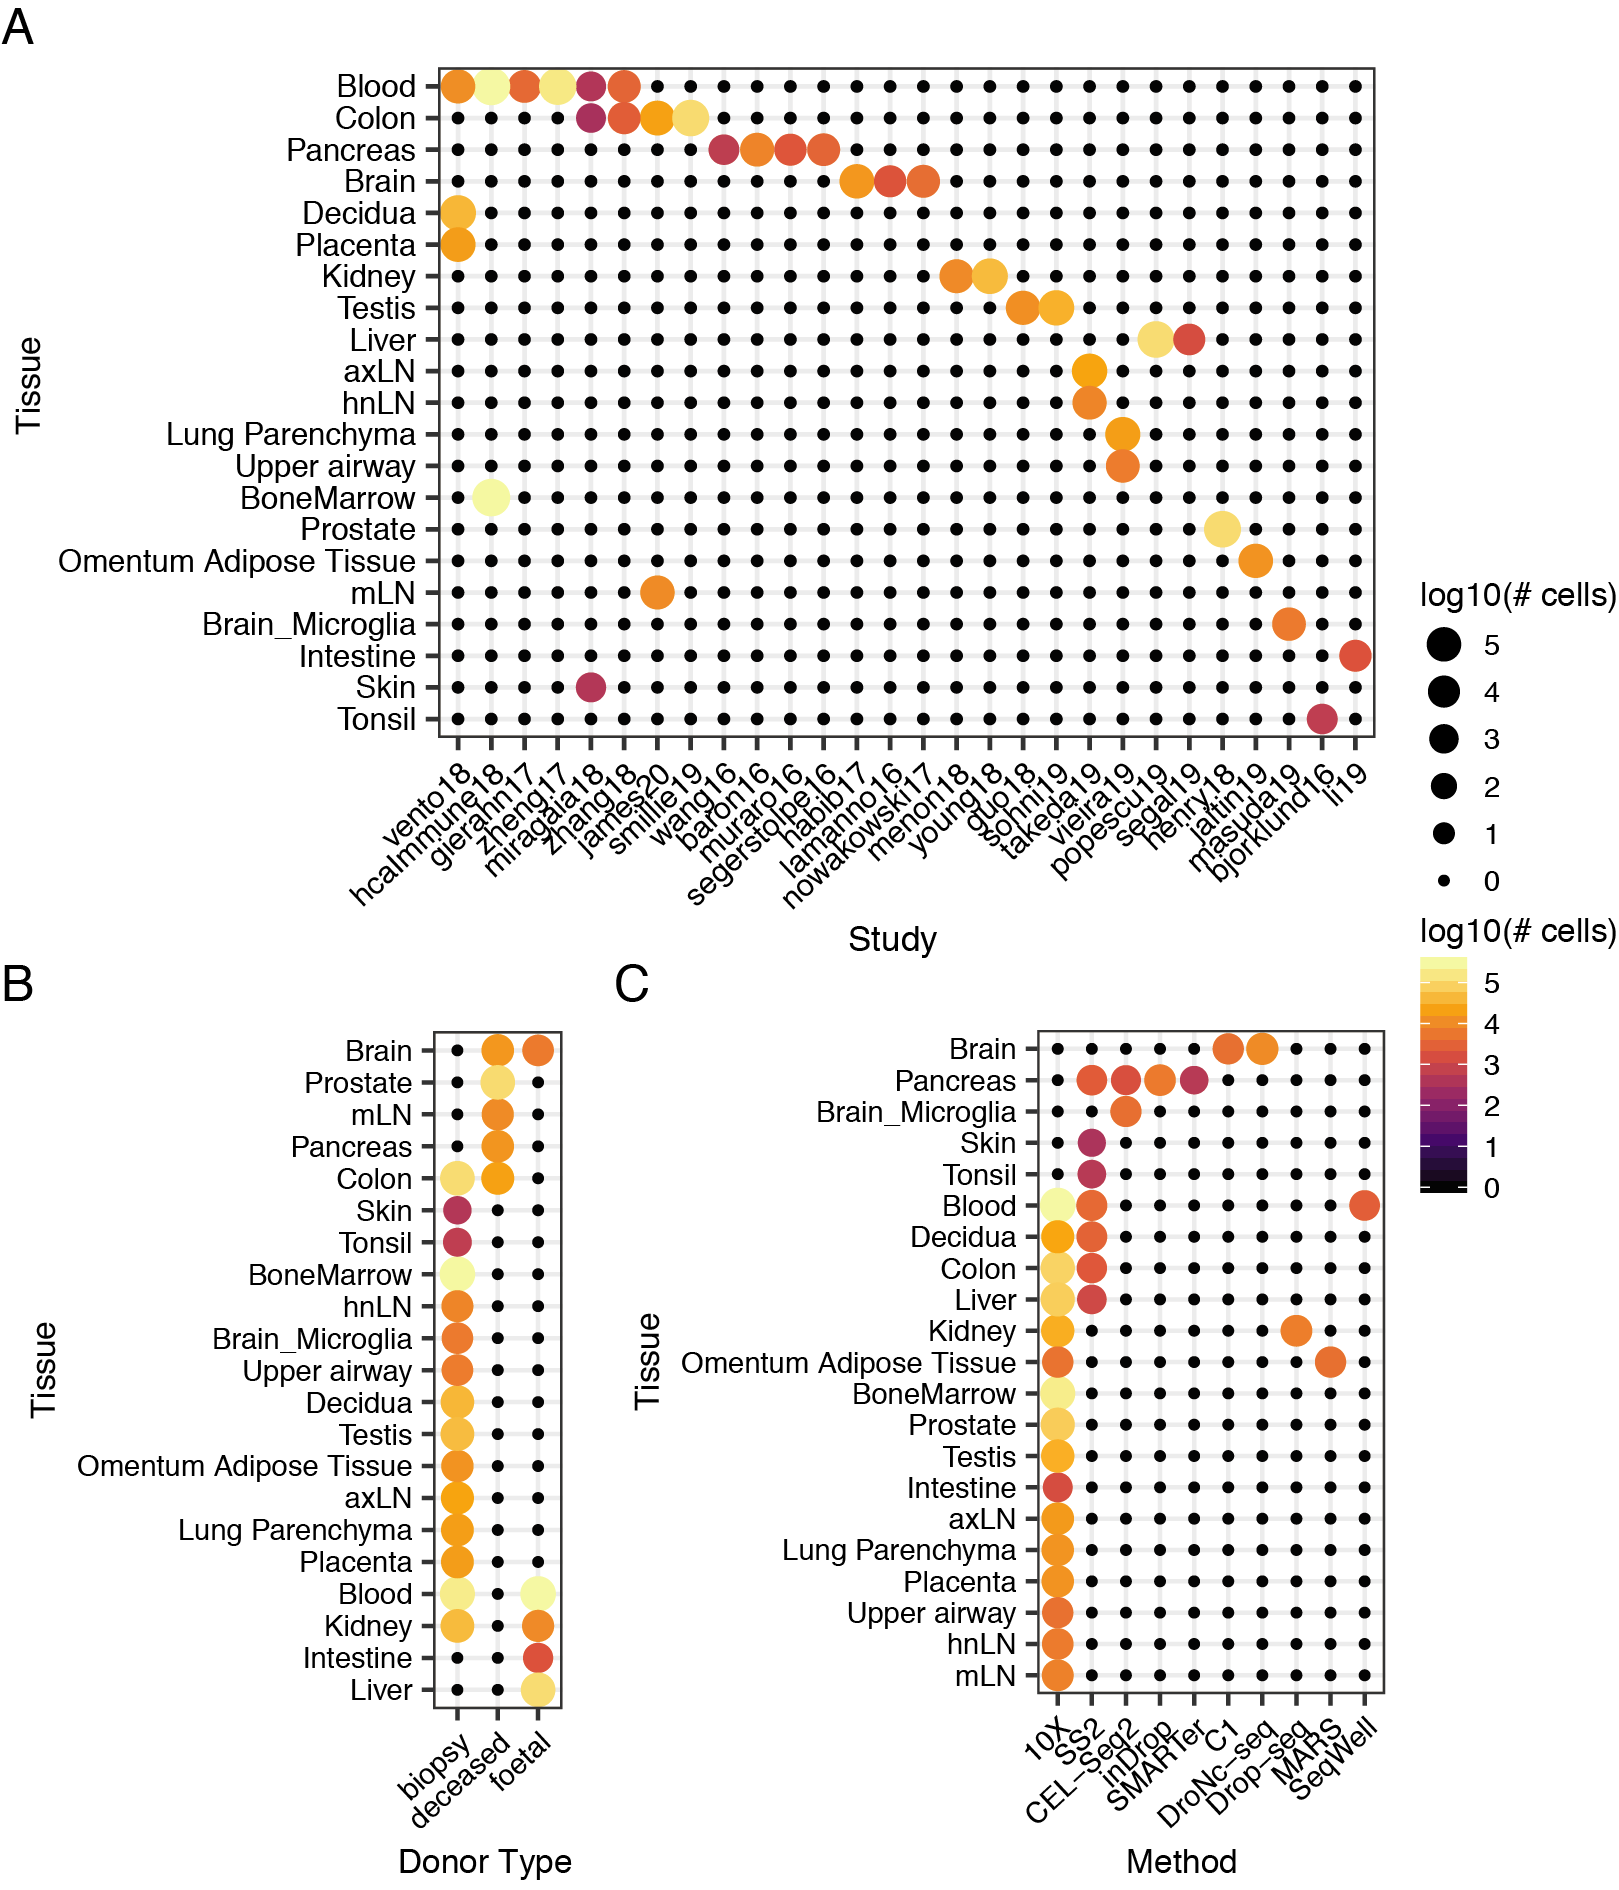
\includegraphics[width=1.0\textwidth]{Chapter4/Figs/chap4_countsHumanAtlas.png} % change word in curlies to change figure
    \caption[Cell numbers in the human dataset collection]{\textbf{Cell numbers in the human dataset collection} \newline Number of cells, in log10 scale, collected from different tissues, and distributed by publication \textbf{(A)}, type of collection \textbf{(B)}, and scRNA-seq protocol \textbf{(C)}.}
    \label{fig:chap4_cha}
\end{figure}

The 28 datasets collected include 21 tissues, mostly collected from adult biopsies (Figure~\ref{fig:chap4_cha}A and ~\ref{fig:chap4_cha}B), and totalling close to 1.5 million cells. Various studies focus on haematopoietic-derived cells, and as such many of the sampled tissues are mostly or completely composed of immune cells. Most cells are obtained using the droplet-based Chromium instrument from 10x Genomics ("10X")



\subsection{TBD}
\label{section4.2_test}



\subsection{Gene expression driving cell identity}
\label{section4.2_genes}



\subsection{Matching cell identity across tissues}
\label{section4.2_tissues}



\section{Discussion}
\label{section4.3}
From its inception, the Human Cell Atlas (HCA) consortium has aimed to "define all human cell types in terms of distinctive molecular profiles (such as gene expression profiles)"~\citep{regev_human_2017}. This task is not one that can be easily accomplished by a single team. Beyond the financial and ethical constraints, collecting good quality scRNA-seq data requires tissue-specific knowledge, as well as profiling using both top-down and bottom-up approaches to obtain an overview of cell populations, while capturing cell type-specific phenotypic variations. Yet as data on human cells accumulates, methods capable of compiling the cellular census envisioned by the HCA members, and make it available to the community will be of great use.

% different studies not properly integrated - but can also be that they have many non-overlapping cell types
%% uniform gene reference problems


% use and availability of this data collection
This large human cell type reference can be very useful to the genomics community the relies on single-cell transcriptome profiling to characterise cell identity in a variety of systems. In disease-focused studies, the steady-state reference provided by \textit{CellTypist} can automatically annotate the cells obtained from a disease sample, eliminating the need to obtain a matching healthy sample. Another potential use is to characterise cell fates and heterogeneity when differentiating organoids. Classifying scRNA-seq data from the generated organoids can reveal the cell types present that a specific protocol was able to differentiate. \textit{CellTypist} will also be available as an online resource, where the model can be directly used, and is accompanied by a database showing the defining characteristics of each cell type - marker genes detected, tissues of origin, datasets characterising them, and similar cell types. This is further intended to be articulated with a Cell Ontology~\citep{bard_ontology_2005}, and have cell names be consistently used when new data is produced, with a direct correspondence to both databases.

% bias in collected data
%% model updating with new data will make it more inclusive/glabally applicable
%% over represented cell types might "hide" smaller ones
%% data augmentation/downsampling can help


% gene biology


%tissue biology


\section{Methods}
\label{section4.4}
\subsection{Single-cell expression data collection}
\label{section4.4_datacol}



\subsection{\textit{CellTypist} training and parameter optimisation}
\label{section4.4_model}



\subsection{Obtaining gene group lists}
\label{section4.4_genelists}



\subsection{Enrichment of gene groups}
\label{section4.4_enr}



